\section{背景}

Random Walk (RW) は図 \ref{Random Walk の概要} に示すように, グラフ上で Random Walker (RWer) が確率 $\alpha$ で終了し, 確率 $1 - \alpha$ でランダムな隣接頂点に遷移するアルゴリズムであり, グラフ解析において広く利用されている. RW を用いたグラフ演算の例として, Personalized PageRank \cite{PPR} (PPR) がある. PPR により, ある頂点から見た他の頂点の関連度を算出することができる. 例えば Web ページを頂点, Webページ間の参照関係をエッジとしたグラフ上で PPR 演算をすることで, Web サイトの推薦システムを作成することができる. 他にも RW は, コミュニティ検出, リンク予測, 類似性推定や機械学習等のアプリケーションで利用される. 

解析対象となるデータは世界中で日々増加し, 各地域のデータセンターに保存される. 例えば, Amazon Web Service は全世界の 33 箇所の地域にそれぞれクラウドインフラストラクチャを保有している \cite{aws} . 世界規模で展開されるサービスの運用のためには, 世界中に分散したデータを解析する必要がある. 図 \ref{地理的分散環境下におけるグラフ} に地理的分散環境下でのグラフ管理のイメージを示す. データセンター 1, 2, 3 が各々部分グラフを管理しており, 一部頂点は異なるデータセンターが保持する頂点へのエッジを持つ. このようなグラフを解析するとき, 中央集権的に全ての部分グラフを一箇所に集めてから解析することが理想だが, 以降に述べる理由によりこれはコストが非常に高い, もしくは実現不可能である. まずグラフの規模が非常に大きく, グラフの変化も頻繁に発生するため, 広域ネットワーク (WAN) での転送コストが高い. また, GDPR のようなプライバシー規制によって, その地域のデータセンターに保存されている元データを転送できない場合も考えられる. そのため, 地理的に分散した環境下におけるグラフ解析 (本研究では RW) のためのシステム開発が重要となる. 

既存の分散グラフ RW 実行エンジン \cite{10.1145/3341301.3359634} は単一のデータセンター内での実行を想定しており, 地理的分散環境下のような RTT, パケットロス率が高い環境では大きく性能が劣化することがわかっている (\ref{RTT, パケットロス率を変えた場合の実行時間} 節参照). この手法ではサーバ間での RWer 送受信に TCP 通信を採用しており, 地理的分散環境下ではスループットが小さくなるためである. また, 既存手法は Bulk synchronous parallel (BSP) モデル (\ref{sec:分散グラフ処理システム} 節参照) による同期処理を行うが, この処理方式は本研究が想定する地理的分散環境下には適さないと考える. まず, 同期処理をする場合サーバ間同期のための通信が何度も発生するが, WAN のような低帯域・高遅延の環境ではこの通信のオーバヘッドが増加する. また, 頻繁なグラフ編集により全体として見たときのグラフ分割精度が悪くなってしまう場合, 負荷不均衡により同期処理における同期待ちが発生する. さらに, 地理的分散環境下での RW 実行エンジンの用途について, 各データセンターが, 自身が保有する頂点を始点とした RWer の生成・ 処理を自律的に行い, その RW 結果をそのデータセンターの所在地域が活用するような地産地消型の自律的 RW 実行が主流になると考えている. 

そこで本研究では, 地理的分散環境下に適した RW 実行エンジンを提案する. 提案手法は, 本手法の用途を意識することに加え, RWer 単位での独立性という RW 演算の特徴に注目し, UDP 通信を使用した非同期処理を採用した. UDP 通信を利用することで, WAN におけるスループットの低下を抑えられる. そして非同期処理を採用することで, 各データセンターによる自律的な RW 実行を実現することができる. また, 提案手法は過去に終了した RWer の経路を再利用することで, RW 遷移時の通信量を削減する機能を有する. 地理的分散環境下を想定した実験によって, 提案手法が既存手法よりも実行時間やグラフ分割精度変化に対する耐性, システム規模に対するスケーラビリティなどの観点で適切な手法であることを明らかにする. 

\begin{figure}[t]
    \centering
    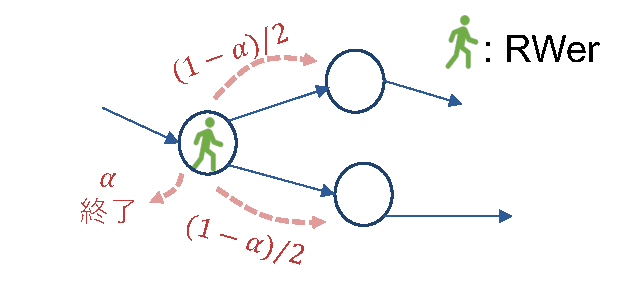
\includegraphics[scale=1.0]{figure/RandomWalk.pdf}
    \caption{Random Walk の概要}
    \label{Random Walk の概要}
\end{figure}

\begin{figure}[t]
    \centering
    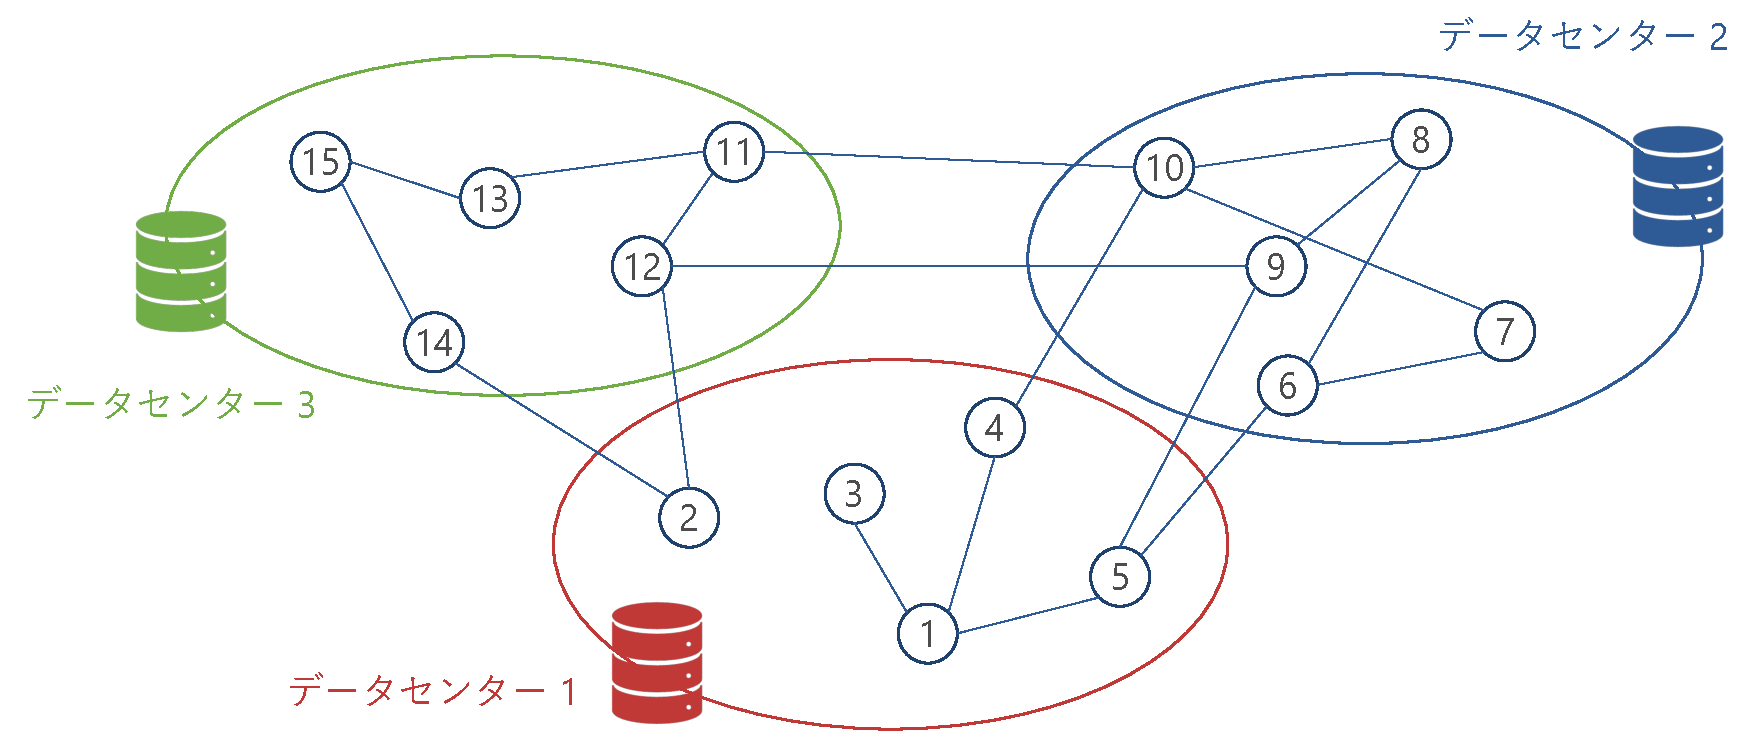
\includegraphics[scale=0.5]{figure/dcgraph.pdf}
    \caption{地理的分散環境下におけるグラフ}
    \label{地理的分散環境下におけるグラフ}
\end{figure}

\section{本論文の構成}

本節にて以降の本論文の構成を示す. まず第 \ref{chap:related_work} 章で関連研究について述べる. 次に第 \ref{chap:design} 章では本研究における提案手法について述べる. 第 \ref{chap:eval} 章では提案手法の評価について述べ, 最後に第 \ref{chap:conclusion} 章で本論文をまとめ, 今後の課題について述べる. 